% Auto-generated snippet: PC2/PC3 analysis
\begin{table}[t]
  \centering
  \caption{Top PC2/PC3 Pearson correlations by absolute effect size.}
  \begin{tabular}{l l r r r}
    \hline
    PC & Variable & $n$ & $r$ & $p_{perm}$ \\
    \hline
    pc3 & electronegativity_pauling & 100 & -0.289 & 0.005199 \\
    pc2 & ionization_energy_1 & 104 & 0.263 & 0.0196 \\
    pc3 & group & 80 & -0.261 & 0.006399 \\
    pc3 & atomic_number & 108 & -0.241 & 0.007998 \\
    pc3 & period & 108 & -0.190 & 0.04699 \\
    pc3 & atomic_radius & 86 & 0.187 & 0.08598 \\
    pc3 & ionization_energy_1 & 104 & -0.120 & 0.1806 \\
    pc2 & atomic_radius & 86 & -0.083 & 0.4589 \\
    \hline
  \end{tabular}
  \label{tab:pc2-pc3-topcorr}
\end{table}

\begin{figure}[t]
  \centering
  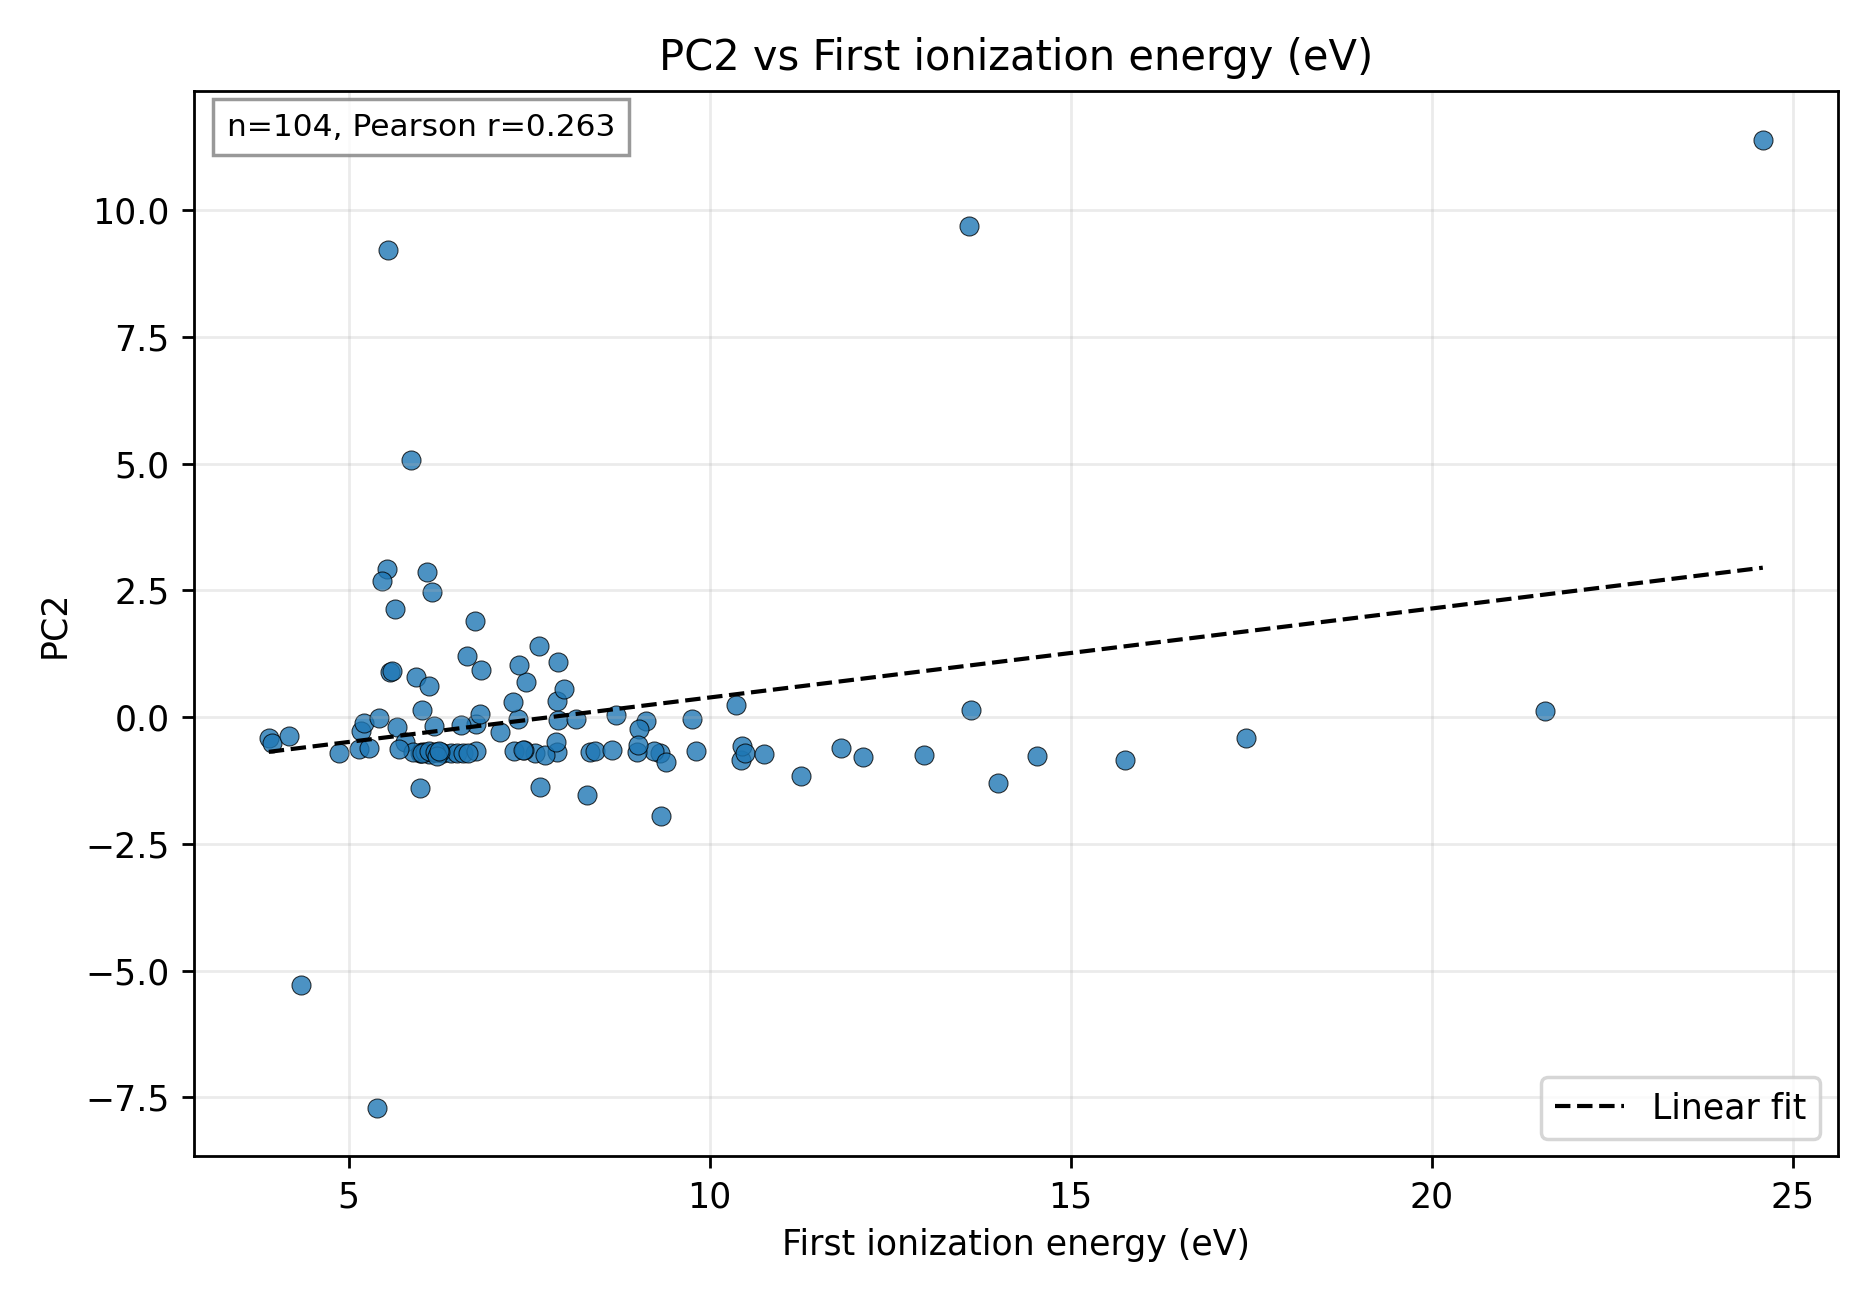
\includegraphics[width=0.82\linewidth]{figures/fig_pc2_vs_period.png}
  \caption{PC2 vs First ionization energy (eV).}
  \label{fig:pc2-ionization_energy_1}
\end{figure}

\begin{figure}[t]
  \centering
  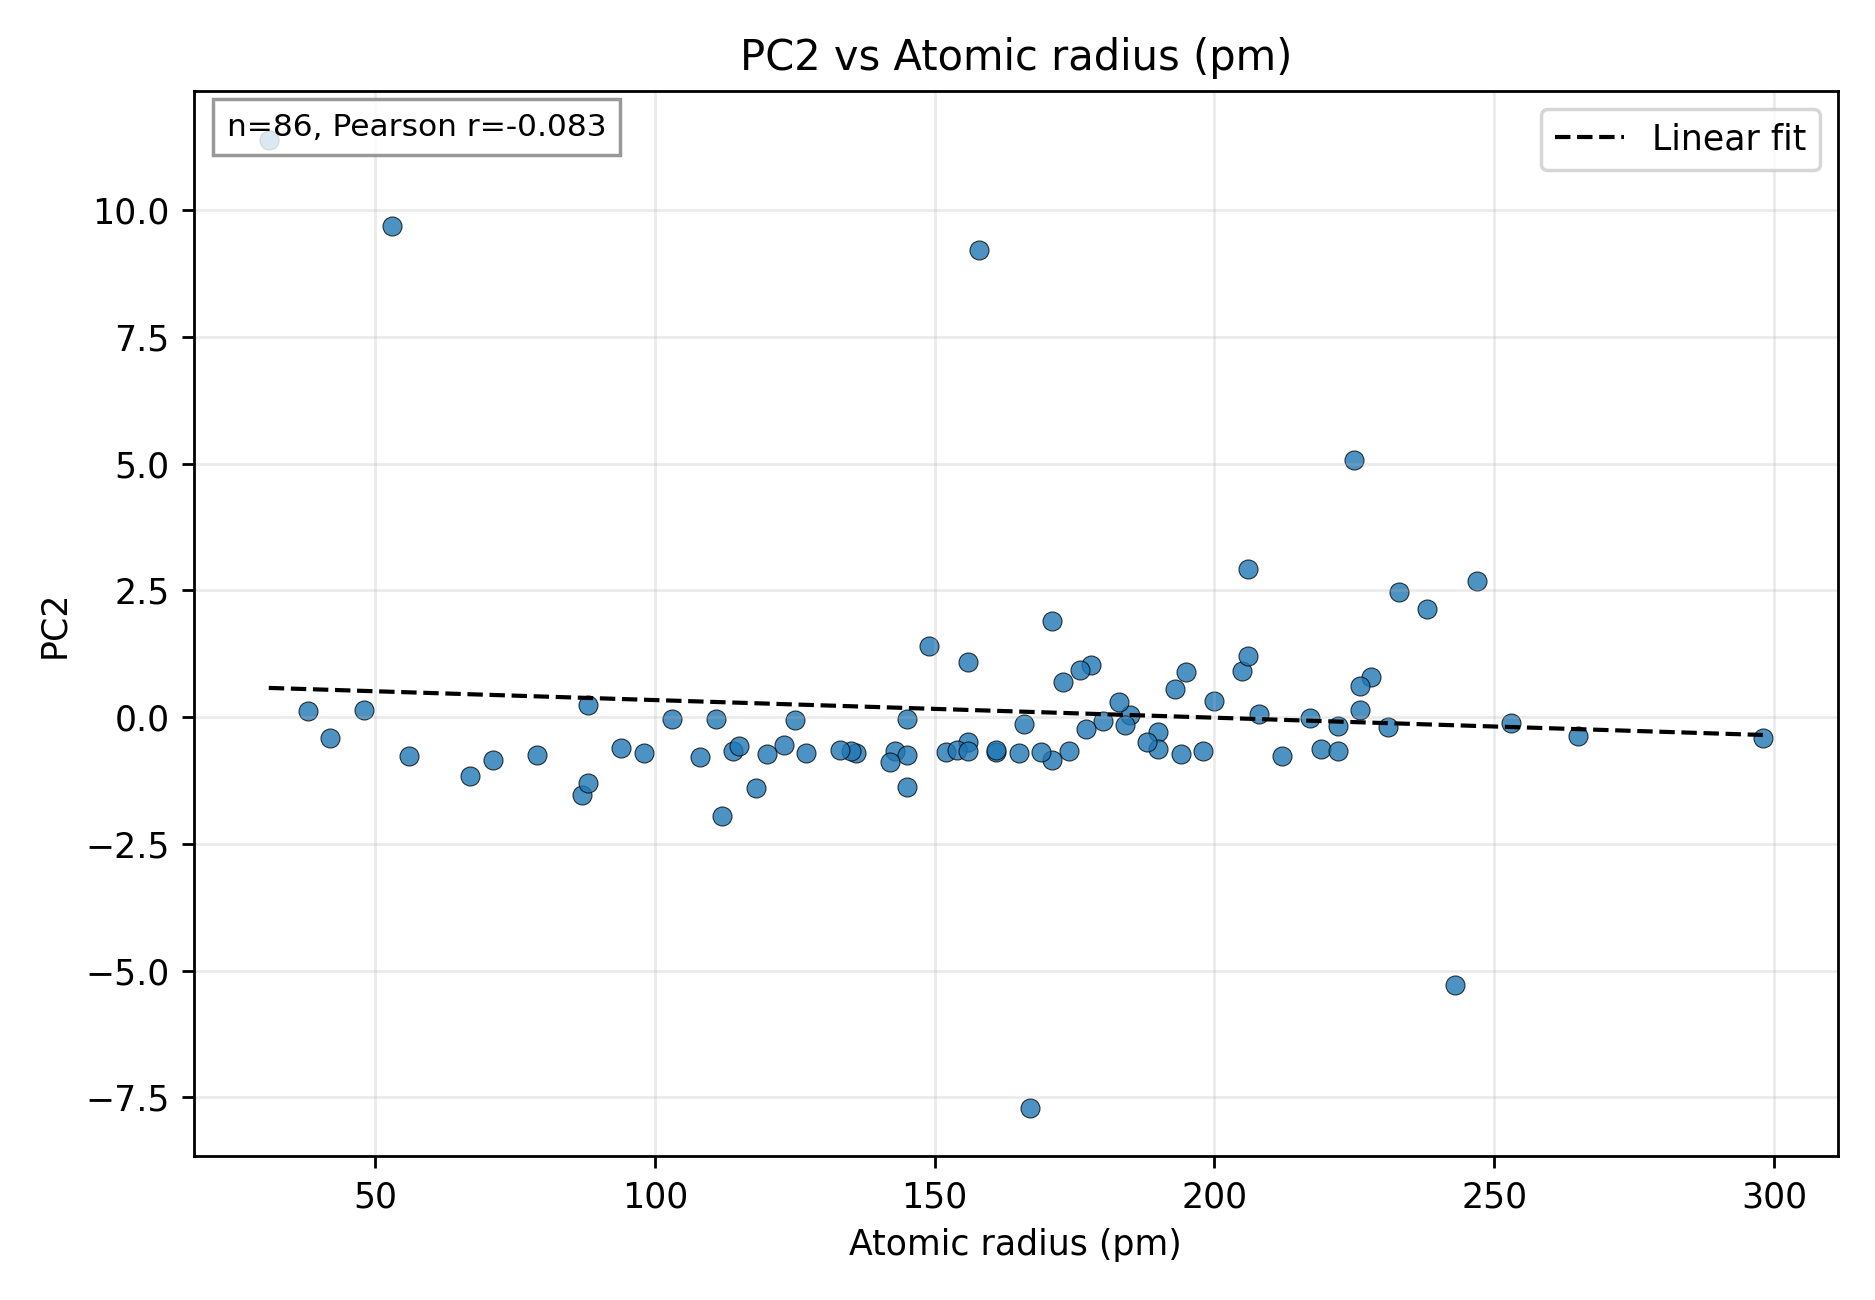
\includegraphics[width=0.82\linewidth]{figures/fig_pc2_vs_ionization.png}
  \caption{PC2 vs Atomic radius (pm).}
  \label{fig:pc2-atomic_radius}
\end{figure}

\begin{figure}[t]
  \centering
  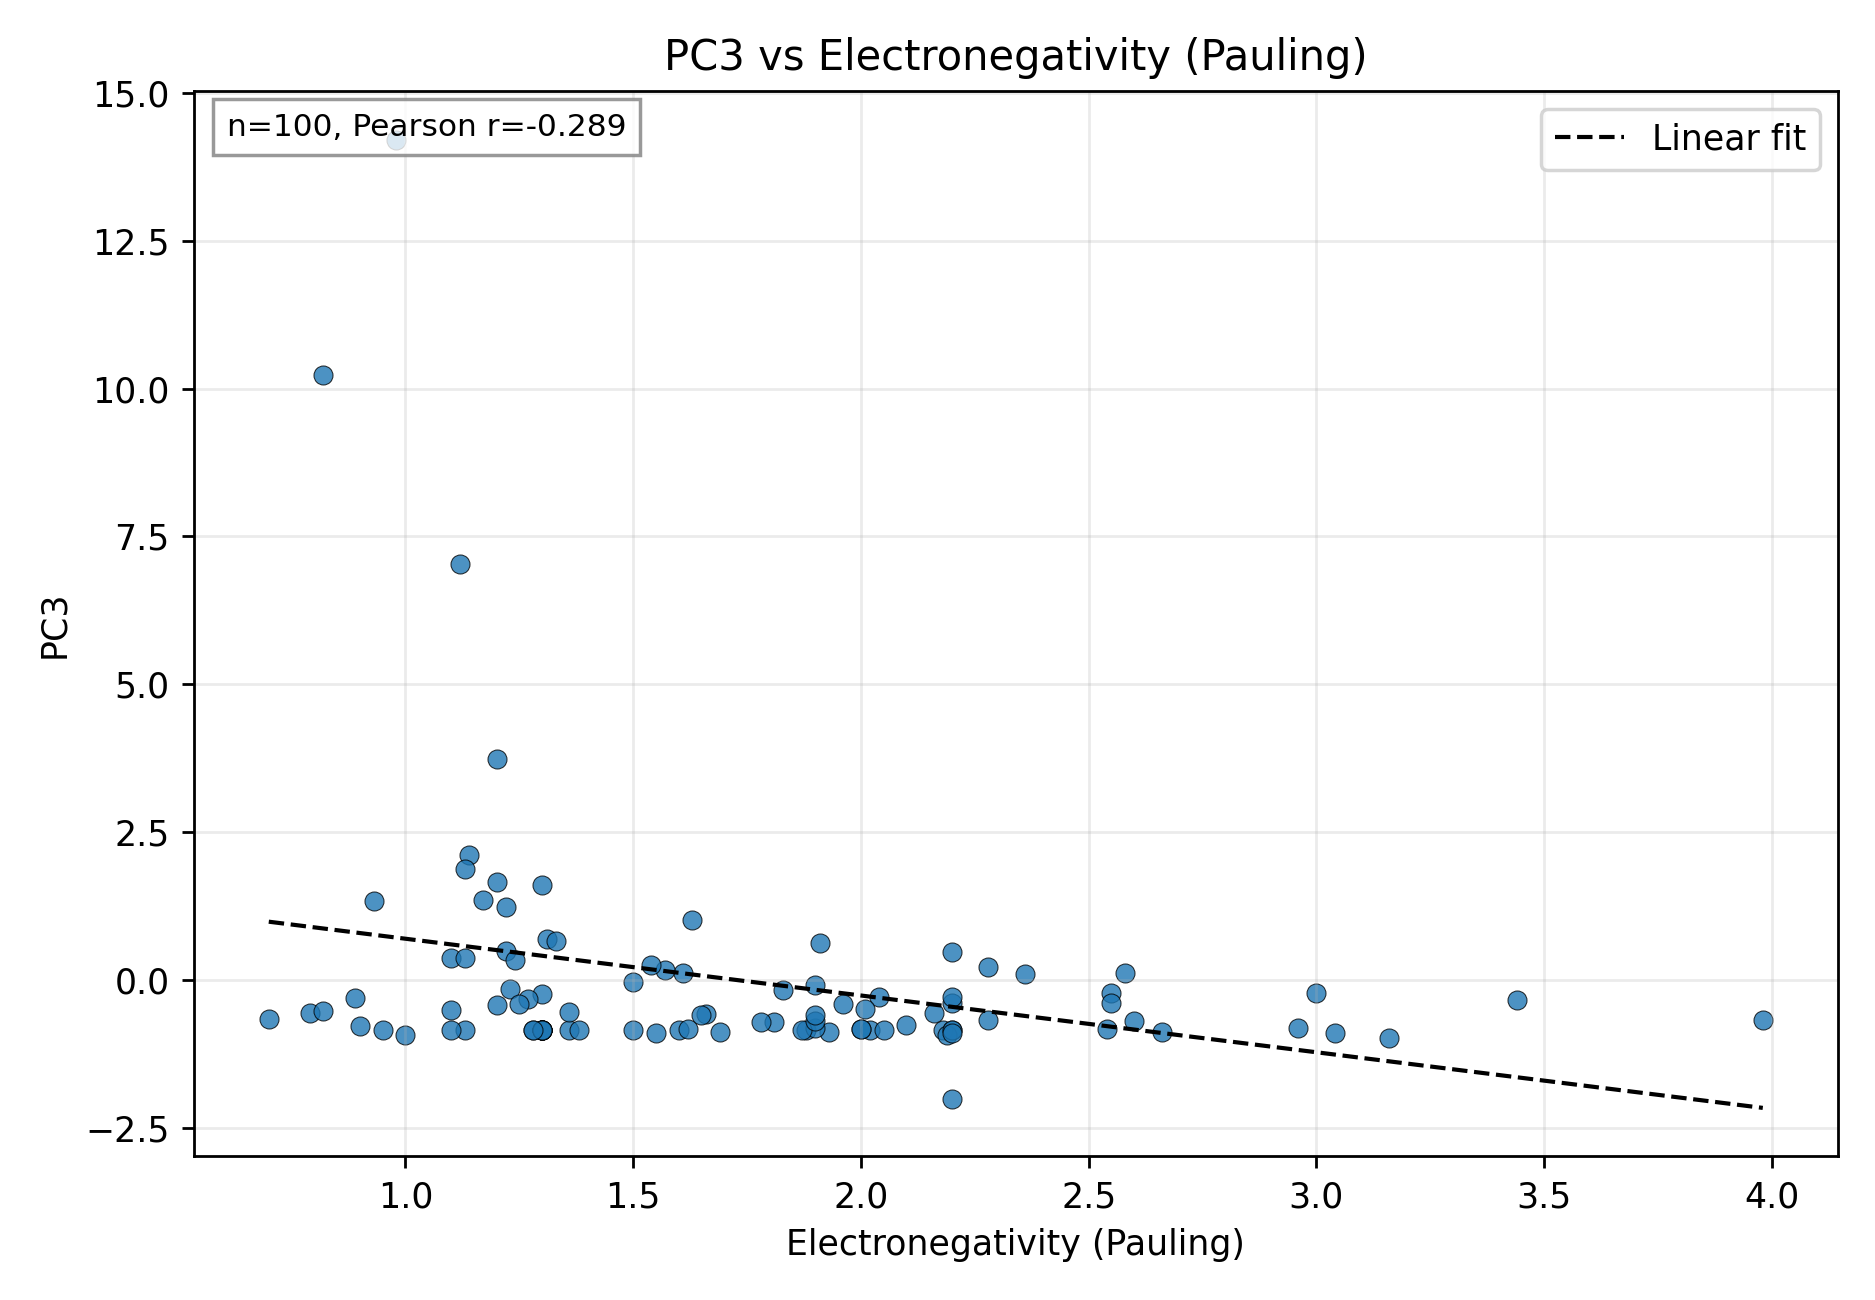
\includegraphics[width=0.82\linewidth]{figures/fig_pc3_vs_period.png}
  \caption{PC3 vs Electronegativity (Pauling).}
  \label{fig:pc3-electronegativity_pauling}
\end{figure}

\begin{figure}[t]
  \centering
  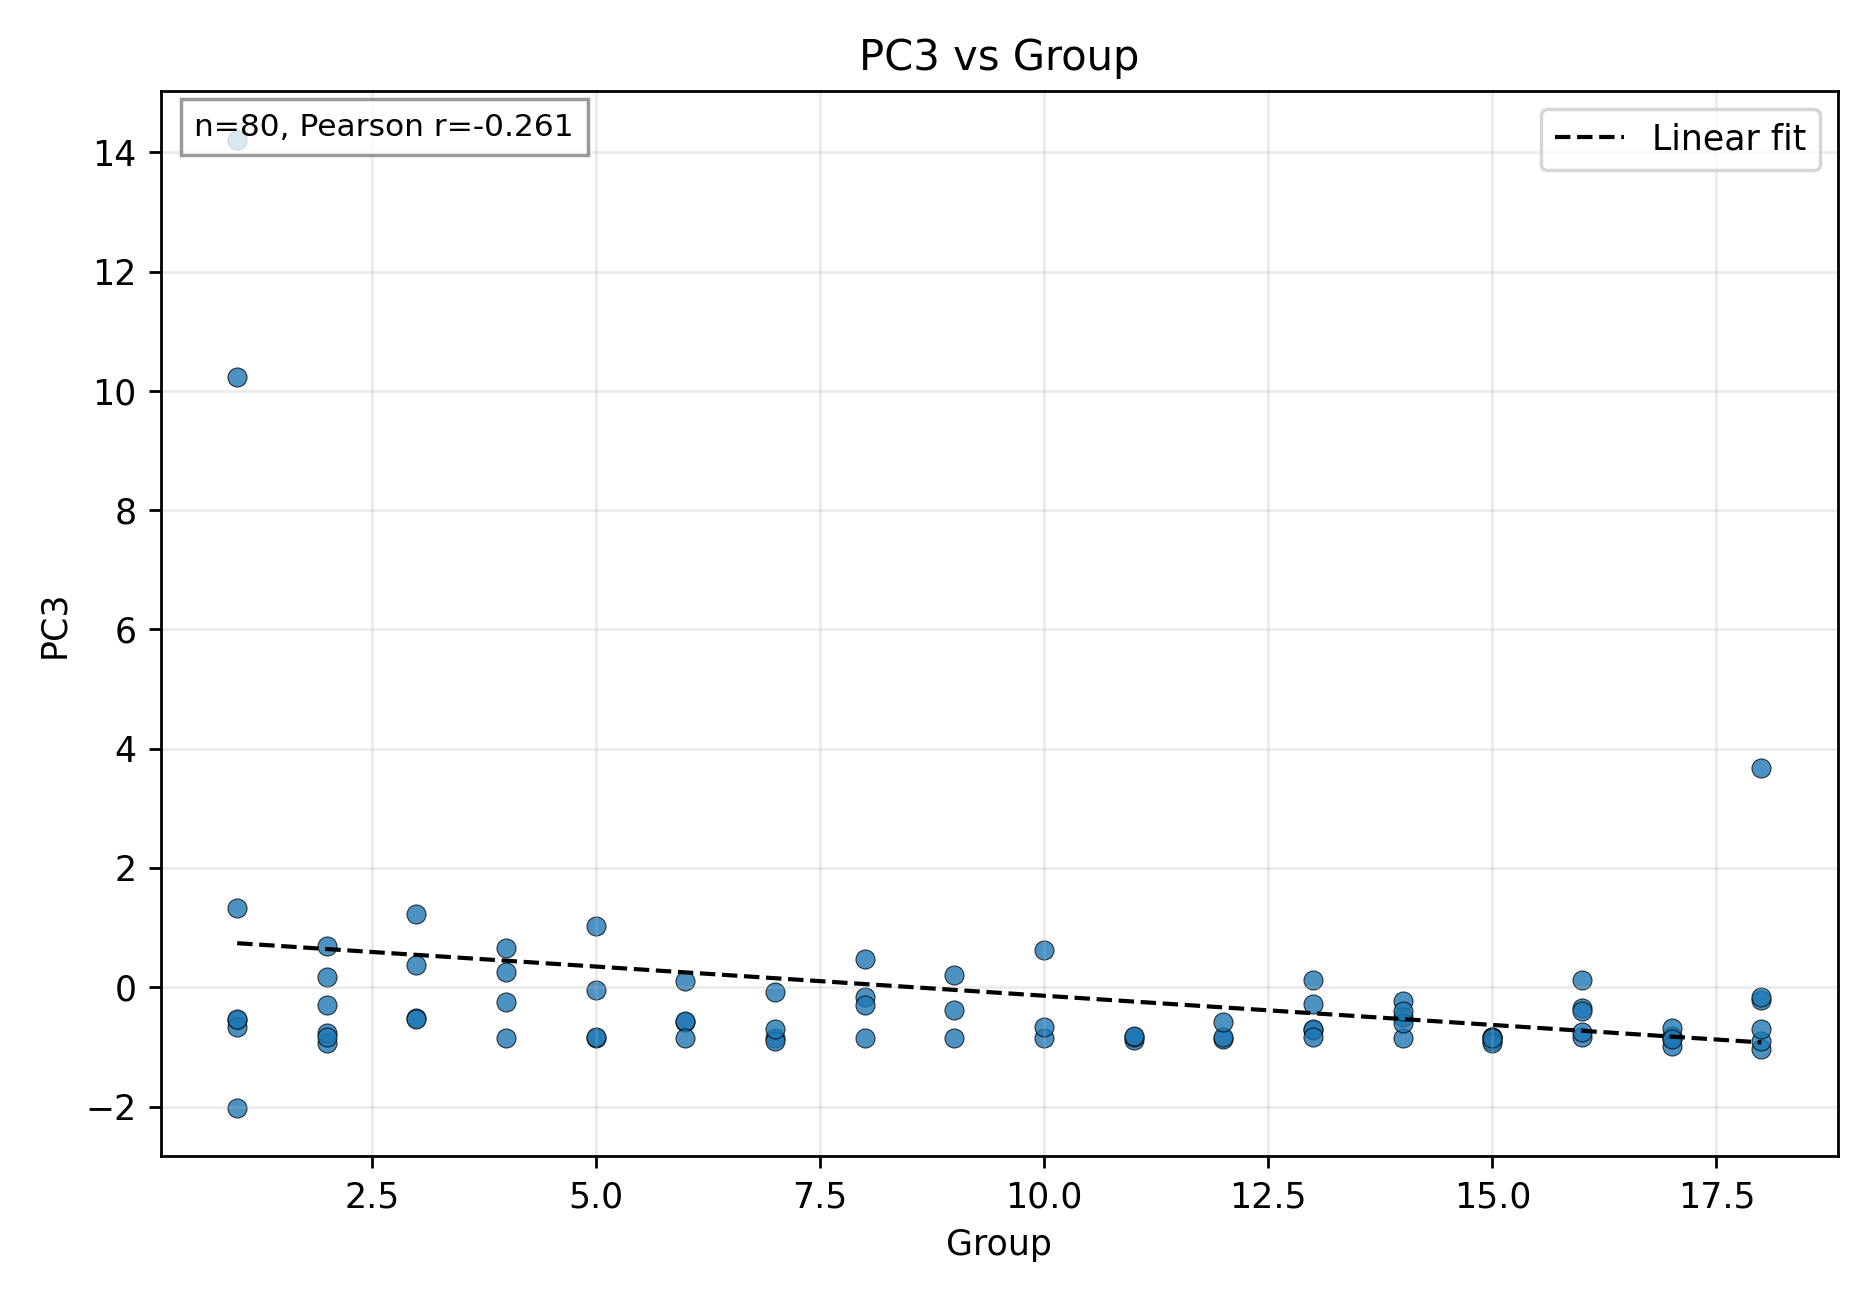
\includegraphics[width=0.82\linewidth]{figures/fig_pc3_vs_radius.png}
  \caption{PC3 vs Group.}
  \label{fig:pc3-group}
\end{figure}

